%!tex root = ../report.tex

\section{Testing Patterns}
In general, there are two ways of testing:
\begin{itemize}
	\item The test is successful if it generates a failure (The goal is falsification of a model)
	\item The test is successful if it does not generate a failure (Commonly used)
\end{itemize}

\subsection{Test Model}
A test model consists of the following components:
\begin{itemize}
	\item \textbf{Test Cases/Tests} Description of the testing activities, derived from use cases
	\item \textbf{Test Driver} Programs executing tests
	\item \textbf{Input Data} needed for the tests
	\item \textbf{Oracle} Compares expected output with actual output of the test
	\item \textbf{Test Harness/Testing Framework} Software components/framework running tests under varying conditions and monitoring behavior
\end{itemize}
\newpage

\subsection{Model-Based Testing}
Model Based Testing is a technique, where the system model is used for the generation of the test model.
This increases the effectiveness of testing, as costs are reduced and maintenance is easier.
Also artifacts such as analysis and design models are reused.
\newline

The platform independent system model can be transformed into the platform independent test model.
The platform specific test model can be derived from the platform specific system model or the platform independent test model.

Model-based testing enables the early integration of testing into the
system development process (test driven development).

\begin{figure}[h!]
	\centering
	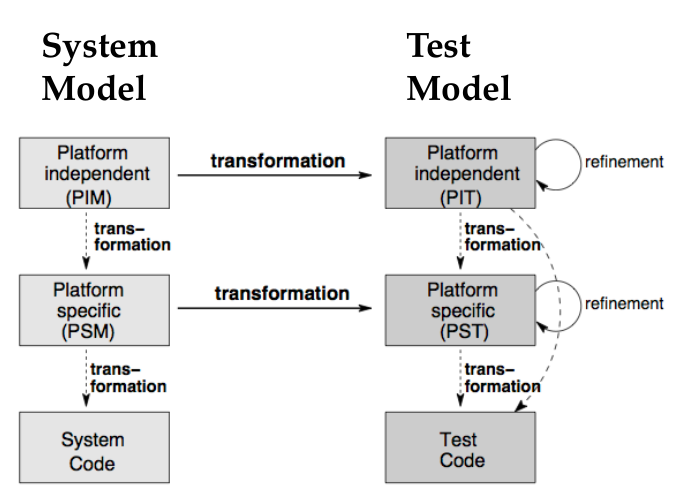
\includegraphics[width=0.8\linewidth]{images/testing_generating_test_code}
	\caption{Transformation from System to Test Model}
\end{figure}
\newpage

\subsection{Testing Activities}
There are different types of testing:
\begin{itemize}
	\item \textbf{Unit Testing/Module Testing} developers test individual components, confirms correct coding of component or subsystem
	\item \textbf{Integration Testing} developers test groups of subsystems, confirm interface specifications of subsystems
	\item \textbf{System Testing} developers test the entire system, checks if system requirements are meet
	\item \textbf{Acceptance Testing} client evaluates the system by executing typical use cases, checks requirements
\end{itemize}

Tests after each change are called \textbf{regression tests}.

\begin{figure}[h!]
	\centering
	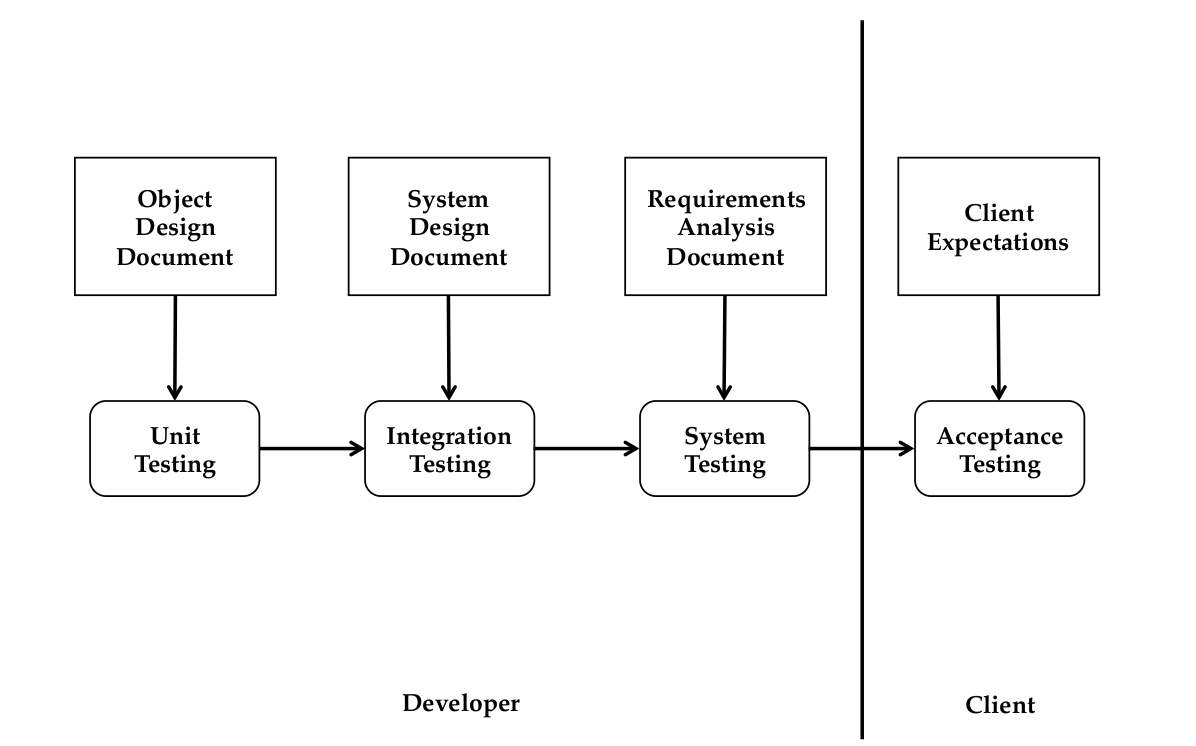
\includegraphics[width=\linewidth]{images/testing_activities}
	\caption{Testing Activities}
\end{figure}
\newpage


\subsection{JUnit Testing}
JUnit is a Java framework for writing and running unit tests to test individual functions.
It consists of test cases and suites, as well as a test runner.


\subsubsection*{Annotations}
\renewcommand{\arraystretch}{1.4}
\begin{tabular}{ll}
	\texttt{@Test public void foo()} & \texttt{foo} is a test \\ \hline
	\texttt{@Before public void bar()} & \texttt{bar} is executed before every test \\ \hline
	\texttt{@After public void foobar()} & Any test method must finish with call to \texttt{foobar} \\ \hline
	\texttt{@BeforeClass public void foofoo()} & \texttt{foofoo} is executed before the start of all tests \\ \hline
	\texttt{@AfterClass public void blabla()} & \texttt{blabla} is executed after all tests have finished \\ \hline
	\texttt{@Ignore(String s)} & Ignores the prefixed method and prints \texttt{s} instead \\ \hline
	\texttt{@Test(expected=IllegalArgumentException)} & Tests if the test method throws the named exception \\ \hline
	\texttt{@Test(timeout=100)} & Test fails, if it takes longer than 100 milliseconds
\end{tabular}
\renewcommand{\arraystretch}{1}

\subsubsection*{Assertions}
\begin{itemize}[]
  \item \texttt{assertTrue(predicate)}
  \item \texttt{assertFalse(predicate)}
  \item \texttt{fail(String)} \textit{lets the method fail, used in code which should be unreachable}
  \item \texttt{assertsEquals([String message], expected, actual)}
  \item \texttt{assertsEquals([String message], expected, actual, tolerance)} \textit{used for float and double}
  \item \texttt{assertNull([message], object)} \textit{prints message if object is null}
  \item \texttt{assertNotNull([message], object)}
  \item \texttt{assertSame([String], expected, actual)} \textit{expected == actual (not equals!)}
  \item \texttt{assertNotSame([String], expected, actual)}
\end{itemize}
\newpage

\subsection{Object-Oriented Model-Based Testing}
The test model now contains \textbf{objects} called doubles (from stunt double) that replace classes in the system that have not yet been implemented.

There are four types of doubles:
\begin{itemize}[topsep=3pt]
  \item \textbf{Dummy Object:} Used to fill parameter holes, never actually used
  \item \textbf{Fake Object:} Functional class, that has not yet the actual functionality of the real class (e.g. database implementation that is stored on the memory only)
  \item \textbf{Stub:} Returns always the same values (e.g. always 42 in a random number generator)
  \item \textbf{Mock Object:} Imitates real behavior of an object. Requires a good architecture to let the mock class inherit from the desired interface.
\end{itemize}
\newpage

\subsubsection{Mock-Object Pattern}
\begin{figure}[h]
  \centering
  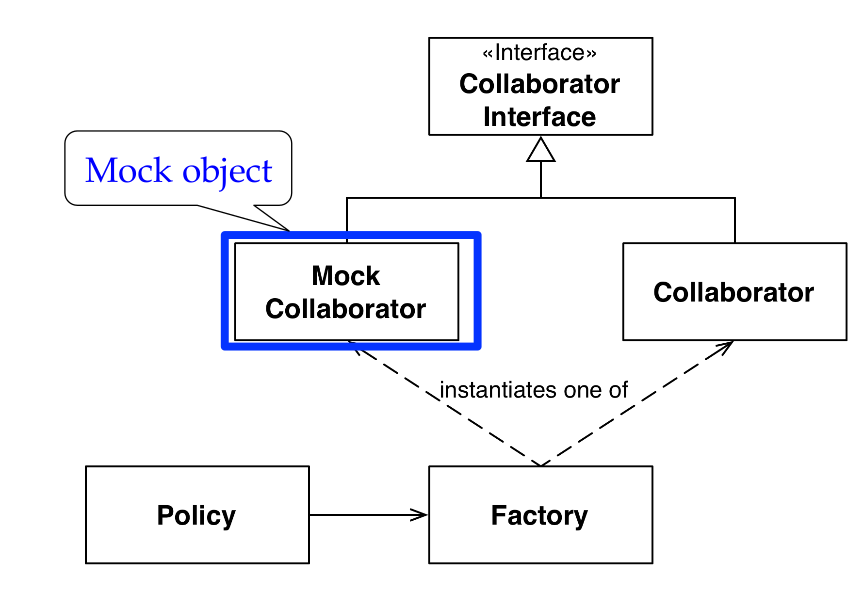
\includegraphics[width=.75\linewidth]{images/testing_pattern_mock_object.png}
  \caption{Structure of the Mock-Object Pattern}
\end{figure}
Applicability:
\begin{itemize}
  \item Unit tests with nondeterministic behavior (e.g. weather)
  \item Object is difficult to set up (e.g. large mazes in a game)
  \item Specific behavior is hard to trigger (e.g. network errors)
  \item Slow methods (e.g. climate modeling)
  \item Object has an user interface or is the user
  \item The real object is not testable
\end{itemize}
Easy Mock:
\begin{enumerate}
  \item Instantiate mock object: mock = createMock(foo.class)
  \item Specify the expected behavior
  \begin{enumerate}
    \item Void methods are called as in Java
    \item For methods with return values: use expect() to specify the return value and andReturn() to specify the expected value
    \item times() defines how often the method can be called
  \end{enumerate}
  \item Use replay(mock) to make the mock object available
  \item Invoke methods in the SUT (system under test)
  \item Make sure the SUT used the mock object as specified with verify(mock)
\end{enumerate}
\newpage

\subsubsection{Dependency Injection Pattern}
Dependency injection is designed to avoid high coupling between test classes and the SUT.\\
Structure:\\
\begin{figure}[H]
  \centering
  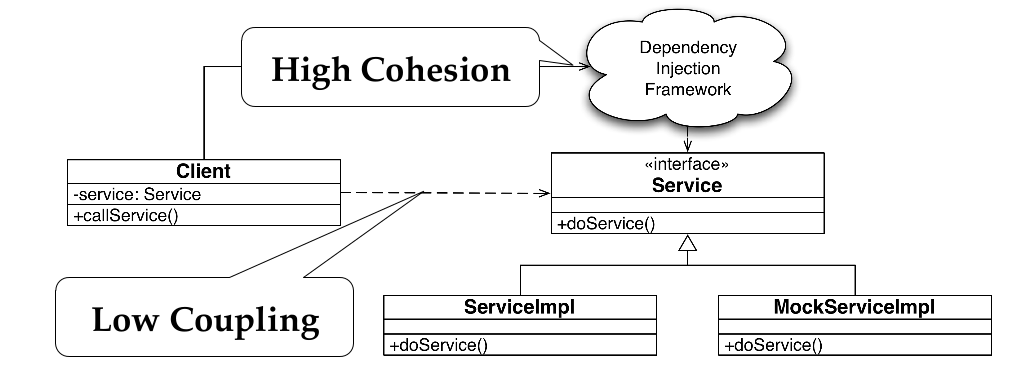
\includegraphics[width=\linewidth]{images/testing_pattern_dependency_injection.png}\\
  \caption{Structure of the Dependency Injection Pattern}
\end{figure}
\textbf{Google Guice Framework:}
\begin{enumerate}
  \item Place the @Inject annotation (constructors, methods, fields)
  \item Create a \textit{Module} to define binding (implement configure()\{bind(Service.class).to(ServiceImpl.class)\})
  \item Instantiate an injector to tell which module to use (Guice.createInjector(new ProductionModule()))
  \item Instantiate an instance of the class needing injection (injector.getInstance(Service.class))
\end{enumerate}
\newpage

\subsubsection{Four-Stage Testing Pattern}
A test driver executes a flow of events to interact with the SUT.
The flow consists of 4 stages:
\begin{itemize}
  \item \textbf{Setup:} Set up the test fixture (initial state).
  \item \textbf{Exercise:} Run tests
  \item \textbf{Validate:} Expected outcome == outcome?
  \item \textbf{Teardown:} Reset the SUT to initial state
\end{itemize}
\newpage

\subsubsection{Testing Pattern for MVC}
\textbf{View-State Test Pattern}\\
Is the view updated when the model changes?\\
\begin{figure}[H]
  \centering
  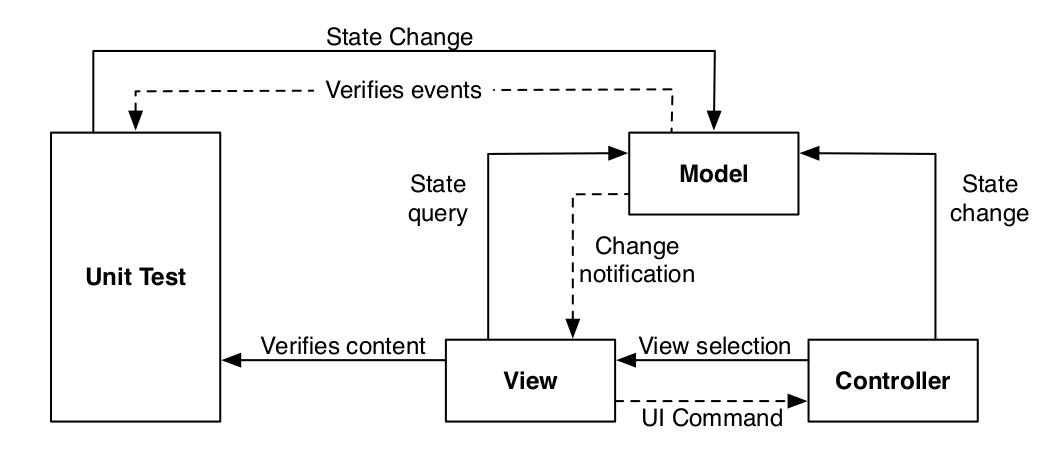
\includegraphics[width=\linewidth]{images/testing_pattern_mvc_view_state.png}
  \caption{Structure of the View-State Test Pattern}
\end{figure}
\textbf{Model-State Test Pattern}\\
Is the model updated when the view is changed via the user?\\
\begin{figure}[H]
  \centering
  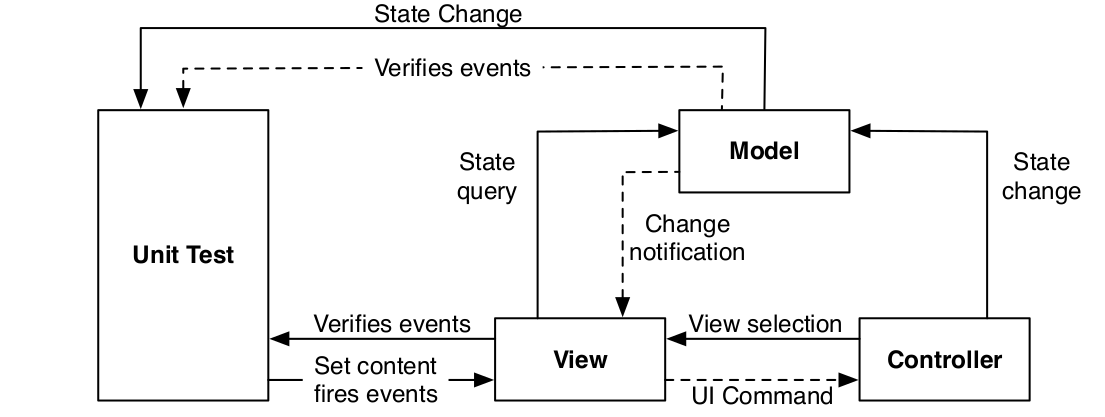
\includegraphics[width=\linewidth]{images/testing_pattern_mvc_model_state.png}
  \caption{Structure of the Model-State Test Pattern}
\end{figure}
\newpage

\subsubsection{Reflection Pattern}
Can be used to test private attributes.\\
\begin{figure}[h]
  \centering
  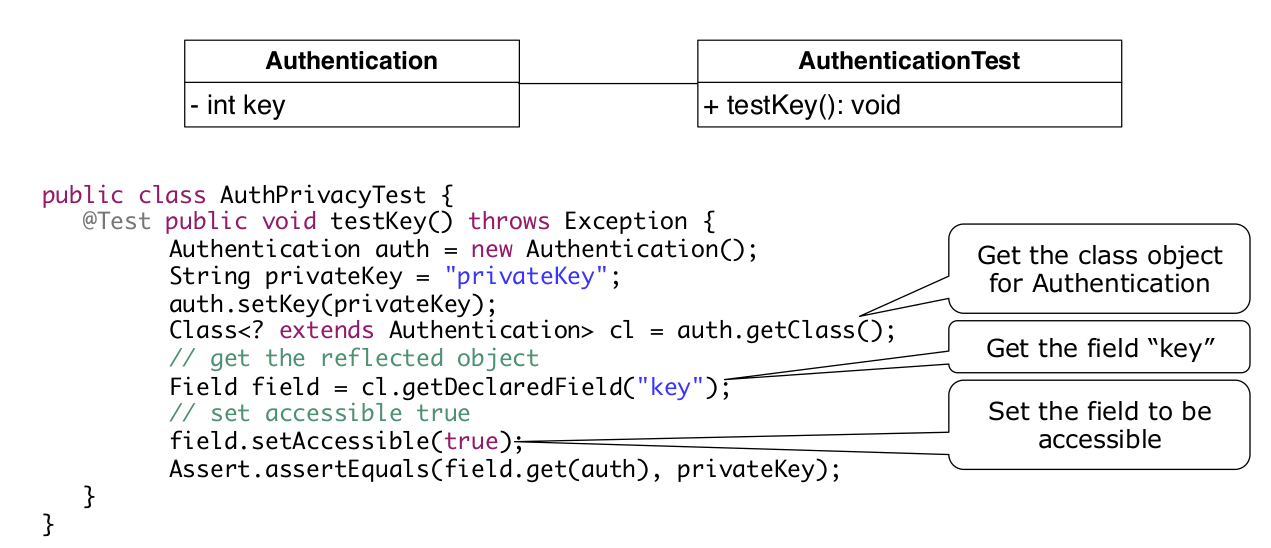
\includegraphics[width=\linewidth]{images/testing_pattern_reflection.png}
  \caption{Example of the Reflection Pattern}
\end{figure}
\newpage
